\documentclass{article}
\usepackage[utf8]{inputenc}
\usepackage[spanish]{babel}
\usepackage{graphicx}
\usepackage{longtable}
\usepackage{float}
\usepackage{amsmath}
\usepackage{listings}
\usepackage{color}

\title{Práctica 4. Parte 2. Algoritmos ByB - Backtracking - Problema del viajante de comercio}

\author{Noelia Escalera Mejías \\
	\and Alejandro Menor Molinero \\
	\and Javier Núñez Suárez \\
	\and Adra Sánchez Ruiz \\
	\and Jesús Torres Sánchez}

\begin{document}
	\maketitle
	\section{Descripción del problema}
	En este caso, hemos propuesto una solución para el problema del viajante de comercio implementando un algoritmo \textit{Branch and Bound}. Además, hemos ejecutado la versión con técnica de \textit{Backtracking} para comparar la eficiencia entre ambos algoritmos.
	
	\section{Cotas global y cota local}
	Para implementar el algoritmo de \textit{Branch and Bound}, necesitamos dos cotas: 
	\\
	
	Por un lado tenemos la \textbf{cota global}, que determina la mínima distancia encontrada hasta el momento para un circuito generado. Si aún no se ha encontrado ninguna solución, estará inicializada de acuerdo a una versión \textit{Greedy} del problema (en este caso, se ha usado la aproximación basada en Inserción).
	
	\
	
	Por otro lado, también necesitamos una \textbf{cota local}, que nos servirá a la hora de comprobar la factibilidad (criterio de poda) y en la extracción de los nodos en la cola, de modo que exploraremos antes los nodos más prometedores.
	\subsection{Cálculo de la cota local}
	La cota local consta de tres sumandos:
	\begin{itemize}
		\item Distancia actual: Para todas las ciudades ya seleccionadas, la suma de la distancia entre ellas (sin cerrar el circuito).
		\item La distancia mínima entre la última ciudad seleccionada y cualquiera de las ciudades no seleccionadas aún.
		\item Para cada ciudad no seleccionada, la mínima distancia entre ella y cualquiera de las otras no seleccionadas o la primera ciudad seleccionada.
	\end{itemize}
	
	\section{Representación de la solución}
	A la hora de representar el problema, hemos usado un TDA $Solucion$, para implementar nuestro algoritmo de \textit{Branch and Bound} de forma más clara y organizada.
	\begin{itemize}
		\item \textbf{Información almacenada en el TDA Solucion}:
		\begin{itemize}
			\item \textit {x}: almacena la solución generada hasta el momento. Se representa por medio de un vector de enteros, de modo que la componente $x_i$ del mismo será la ciudad iésima que visitaremos. 
			\item \textit {n}: es el número de ciudades.
			\item \textit{distancias}: representadas con una matriz, en la que cada elemento d[i][j] tiene asociado la distancia entre la ciudad i y la ciudad j. Por tanto, deben coincidir d[i][j] con d[j][i].
			\item \textit {cotaLocal}: contiene la cota local de acuerdo a las ciudades seleccionadas hasta el momento. La hemos descrito con más detalle en la sección anterior.
			\item \textit {distanciaActual}: es la distancia acumulada para las ciudades ya seleccionadas hasta el momento. 
			\item \textit {ciudadesYaSeleccionadas}: representadas como un vector de booleanos, su componente $x_i$ será $true$ si la ciudad $i$ está ya seleccionada y por tanto almacenada en el vector solucion $x$.
			\item \textbf{Atributos de clase}
			\begin{itemize} 
			\item \textit {mejorSolución}: es un vector de $n$ elementos que representa la mejor solución encontrada hasta el momento. Este valor se inicializa a partir de una solución Greedy del problema.
			\item \textit {cotaGlobal}: almacena la distancia de la mejor solución descrita en el apartado anterior.
			\end{itemize}
		\end{itemize}
		\item \textbf{Operaciones del TDA Solucion}:
		\begin{itemize}
			\item \textit {Constructor}: realiza una serie de operaciones:
			\begin{itemize}
				\item Inicializa las variables del TDA a sus valores por defecto. Debemos tener en cuenta que, a la hora de inicializar la matriz distancias, el primer elemento es el $d[1][1]$, por lo que debemos añadirle una fila y columna basura para poder acceder con índices que empiecen por 1.
				\item Seleccionamos en primer lugar la ciudad 0 para no generar soluciones equivalentes y reducir así el número de nodos hoja de $n!$ a $(n-1)!$.
			\end{itemize}
			\item \textit {factible()}: únicamente comprueba si la cotaLocal es menor que la cotaGlobal. No es necesario comprobar si el hijo estaba ya seleccionado o no, ya que esto se garantiza por la implementación de nuestra función $generaHijos()$.
			\item \textit {generaHijos()}: este método devuelve un vector con todos los hijos del nodo que lo ejecuta, al añadir cualquiera de las ciudades \textbf{no seleccionadas} al vector solución. En el caso de que a la solución generada le falte solamente una ciudad (y la primera), se completa con la ciudad en cuestión. Actualizamos correctamente los atributos de los nodos hijos (ciudadesYaSeleccionadas, distanciaActual, cotaLocal, etc...)
			\item \textit{actualizarCotaLocal()}: Se llama desde $generaHijos()$ en caso de que no quede sólamente una ciudad más por añadir (como hemos explicado antes), hemos escrito esta función para extraer la lógica del método $generaHijos()$ y poder hacer un poco más mantenible el código.
			\item \textit{esSolucion()}: devuelve si hemos llegado a una solución, es decir, si el tamaño del vector solución coincide con el número de ciudades a explorar. En ese caso, siempre se actualiza la cota global y la mejor solución encontrada. Esto es así, porque en nuestro algoritmo ByB, comprobamos la factibilidad al sacar el nodo de la cola, y antes de llamar a $esSolucion()$. 
			De esta forma, si es factible y es solución, significa que es una solución mejor que la mejor encontrada, ya que en la variable cota local se almacena la distancia real si es un nodo hoja.
			\item \textit{operator 'menor que'}: necesario para almacenar ordenádamente las soluciones en la cola con prioridad que utilizamos en el algoritmo ByB. Para explorar primero los nodos más prometedores, estos se ordenan en la cola de forma ascendente en función de su cota local.
			\item \textit{inicializarCotaGlobal}: inicializa la cotaGlobal y la mejorSolucion a mediante una solución Greedy del problema (en nuestro caso, hemos usado la aproximación basada en Inserción).
			\item \textit{obtenerSoluciónÓptima}: devuelve la solución óptima.
		\end{itemize}
	\end{itemize}

	\section{Algoritmo ByB}
	El algoritmo Branch and Bound sigue el siguiente esquema:
	
	\begin{lstlisting}
void branchAndBound (Solucion sol){
  priority_queue<Solucion> cola;
  cola.push(sol);
  bool fin = false;
  n_nodos = tamq = npoda = 0;

  while (!cola.empty() && !fin){
	Solucion enodo = *cola.begin();
	cola.pop();

	fin = !enodo.factible();

	if (!fin){
		vector<Solucion> hijosDelEnodo = 
				enodo.generaHijos();

		for (Solucion hijo : hijosDelEnodo){
			if (hijo.factible()){
				if (!hijo.esSolucion())
				   cola.push(hijo);
			}
			else
				npoda++
		}
	}
	else
		npoda += cola.size();
	if (cola.size() > tamq)
		tamq = cola.size();
		
	n_nodos++;
  }
}
	\end{lstlisting}
	
	\section{Estudio empírico}
	Hemos decidido comparar ambos algoritmos ya no solo en implementación, sino también en tiempo. He aquí una comparativa de los tiempos en los distintos mapas:
	
	\begin{longtable}{|c|c|c|}
		\hline
		Mapa & Branch \& Bound & Backtracking \\ \hline
		Ulysses10 & 0.0561154 & 0.032728  \\ \hline
		Ulysses14 & 27.554 & 38.1479 \\ \hline
		Burma14 & 2.30142 & 4.7288\\ \hline
		Ulysses16 & 745.77 & 1232.72\\ \hline
	\end{longtable}

	También hemos hecho un estudio del número de podas y nodos expandidos en los distintos mapas con el algoritmo Branch \& Bound.
	
	\begin{longtable}{|c|c|c|c|}
		\hline
		Mapa & Nodos expandidos & Tamaño máximo de la cola & Número de podas \\ \hline
		Ulysses10 & 1937 & 1673 & 6227  \\ \hline
		Ulysses14 & 655875 & 378692 & 3050716 \\ \hline
		Burma14 & 45714 & 18446 & 248076 \\ \hline
		Ulysses16 & 13504373 & 10020741 & 71153628 \\ \hline
	\end{longtable}

	Para obtener el número de podas, simplemente hemos usado una variable \textit{npoda} que se incrementa en una unidad cuando encontramos un hijo no factible y que se incrementa en el tamaño de la cola de prioridad cuando encontramos el mejor nodo de ésta y no es solución. Esto último ocurre ya que cuando sacamos de la cola el nodo más prometedor y este tiene una cota local mayor que la global, no tiene sentido seguir explorando, entonces todos los nodos restantes de la cola que no son explorados son podados también.
	\
	
	Para obtener el número de nodos expandidos hemos usado una variable \textit{n\_nodos} que se incrementa en una unidad cada vez que exploramos un nuevo nodo.
	
	\
	
	Por supuesto, también hemos dibujado las diferentes soluciones a los mapas, he aquí los circuitos hallados:
	
	\begin{figure}[H]
		\centering
		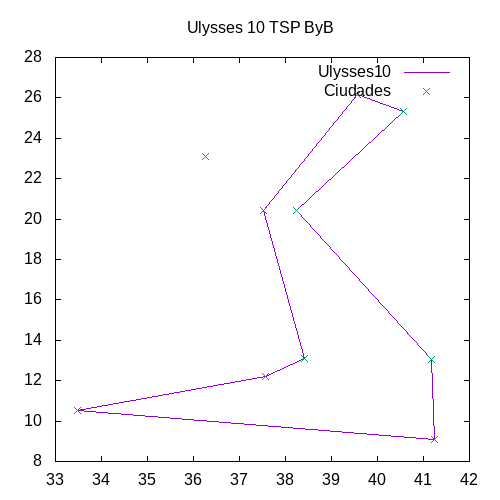
\includegraphics[totalheight=6cm]{ulysses10byb}
		\caption{Circuito Ulysses 10 con Branch \& Bound. Distancia: 45}
		\label{fig:u10byb}
	\end{figure}

	\begin{figure}[H]
		\centering
		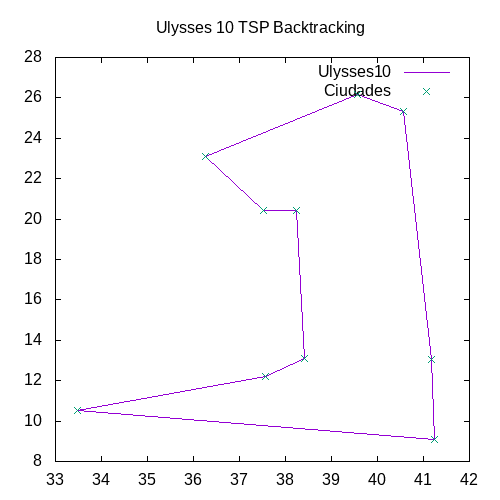
\includegraphics[totalheight=6cm]{ulysses10back}
		\caption{Circuito Ulysses 10 con Backtracking. Distancia: 45}
		\label{fig:u10back}
	\end{figure}

	\begin{figure}[H]
		\centering
		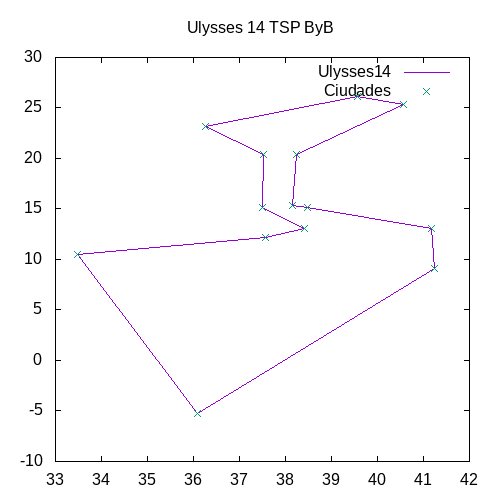
\includegraphics[totalheight=6cm]{ulysses14byb}
		\caption{Circuito Ulysses 14 con Branch \& Bound. Distancia: 68}
		\label{fig:u14byb}
	\end{figure}

	\begin{figure}[H]
		\centering
		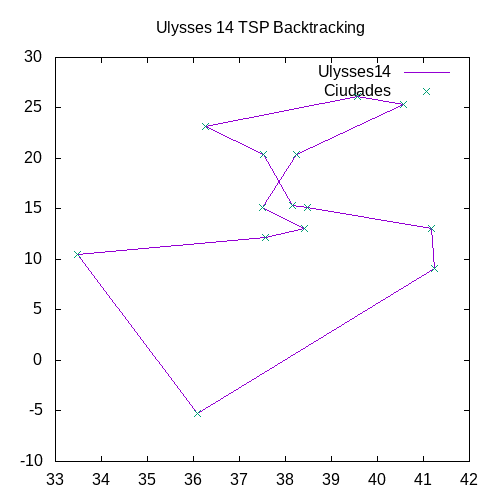
\includegraphics[totalheight=6cm]{ulysses14back}
		\caption{Circuito Ulysses 14 con Backtracking. Distancia: 68}
		\label{fig:u14back}
	\end{figure}

	\begin{figure}[H]
		\centering
		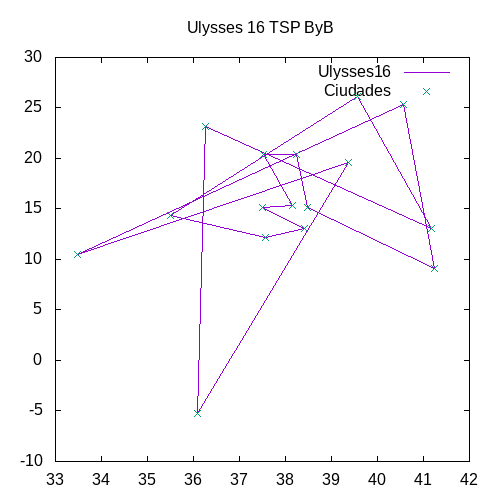
\includegraphics[totalheight=6cm]{ulysses16byb}
		\caption{Circuito Ulysses 16 con Branch \& Bound. Distancia: 71}
		\label{fig:u16byb}
	\end{figure}

	\begin{figure}[H]
		\centering
		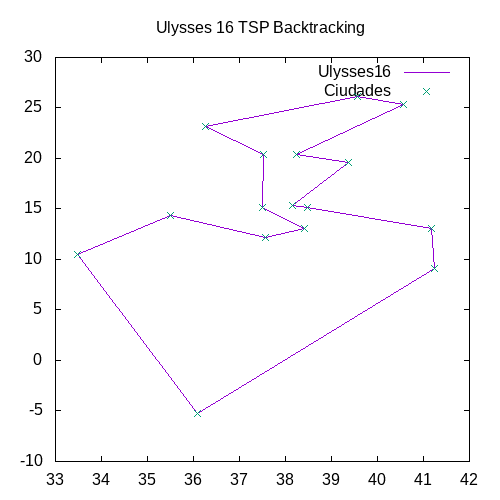
\includegraphics[totalheight=6cm]{ulysses16back}
		\caption{Circuito Ulysses 16 con Backtracking. Distancia: 71}
		\label{fig:u16back}
	\end{figure}

	\begin{figure}[H]
		\centering
		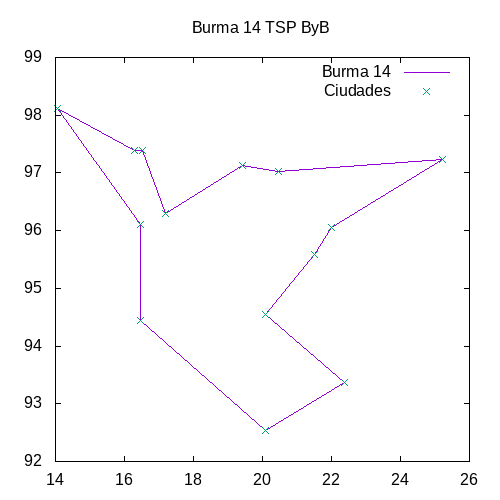
\includegraphics[totalheight=6cm]{burma14byb}
		\caption{Circuito Burma 14 con Branch \& Bound. Distancia: 30}
		\label{fig:b14byb}
	\end{figure}

	\begin{figure}[H]
		\centering
		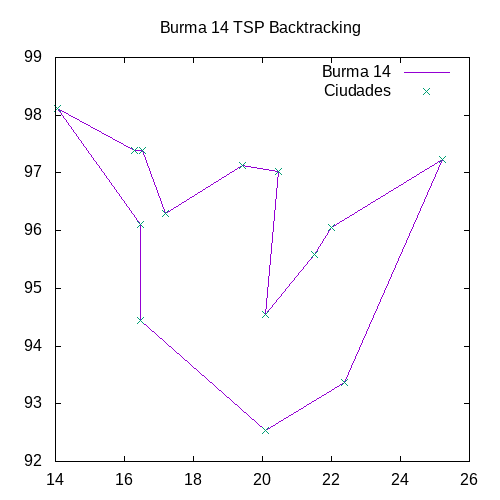
\includegraphics[totalheight=6cm]{burma14back}
		\caption{Circuito Burma 14 con Backtracking. Distancia: 30}
		\label{fig:b14back}
	\end{figure}

	\section{Algoritmo Backtracking VS ByB}
	Como vemos en el estudio anterior, al explorar ramas más prometedoras, el algoritmo Branch \& Bound nos da unos tiempos mucho más bajos. No obstante, la complejidad en espacio es mucho mayor. Como ambos algoritmos encuentran una solución óptima, la distancia del circuito es la misma para ambos recorridos, aunque en algunos casos no se halle el mismo camino.
	
\end{document}